In utilizing access to predictions, a natural algorithm to first consider is one that simply \textit{follows the predictions}. We therefore present algorithm \ref{alg:naive}, which is the main subject of this section.

\begin{algorithm}
\caption{\texttt{Naive}}\label{alg:naive}
\begin{algorithmic}
\State On the arrival of $I$:
\State $I_{s} \gets $ Set of intervals currently in the solution conflicting with $I$
\If{$Prd(I) = 1$ and $I_{s} = \emptyset$}
    \State Take $I$
\EndIf
\end{algorithmic}
\end{algorithm}
\textbf{Unit weights.} We first consider the case of unit weights, and prove the following (positive) result on the performance of algorithm \texttt{Naive}.




\begin{theorem}
    Algorithm Naive achieves $ALG \geq OPT - \eta$ for interval selection with unit weights.
    \label{theo:unw-naive-pos}
\end{theorem}
\begin{proof}
The proof works by mapping optimal intervals to error, and to intervals taken by the algorithm, given that every missed optimal interval can be associated with at least one unit of error. Let $OPT$ be an optimal solution, and let $ALG$ be the algorithm's solution. For each unit of error, we define an error element $h$.
Let $H=\{h_{1},...,h_{\eta}\}$ be the set of error elements. Let $H_{I} \subseteq H$, be the set of error elements corresponding to the error $\eta(I)$. It holds that $H_{I} \cap H_{J} = \emptyset$ for any two distinct intervals $I,J$, and $\bigcup\limits_{I} H_{I} = H$.\\\\
We define an injective mapping $F: OPT \rightarrow ALG \cup H$ as follows: Let $I_{opt}$ be an optimal interval. If $I_{opt}$ is taken by the algorithm, it is mapped onto itself. If $I_{opt}$ is not taken by the algorithm, there are two possibilities. The first possibility is that $Prd(I_{opt}) = 1$, but $I_{opt}$ conflicted with another interval $I_{c}$ taken by the algorithm. For $I_{c}$ to have been taken, it means that $Prd(I_{c}) = 1$, and $|H_{I_{c}} \cup \{I_c\}|>0$ because $I_c$ conflicts with $I_{opt}$. In this case we map $I_{opt}$ to an error element $h_{c}\in H_{I_{c}}$, or $I_c$ itself. Even if more optimal intervals were not taken because they conflicted with $I_{c}$, there will be enough distinct elements in $H_{I_{c}} \cup \{I_c\}$ to map them to.\\\\
The second possibility is that $I_{opt}$ was not taken, because $Prd(I_{opt}) = 0$. In this case, we have that $|H_{I_{opt}}| = 1$, and we can map $I_{opt}$ to the error element of its own prediction. In conclusion, we have that $ALG + |H| \geq OPT$, and we get the desired bound.    
\end{proof}
\begin{corollary}
Algorithm Naive is $1$-consistent.
\end{corollary}

\begin{theorem}
    For every deterministic algorithm, there exist a unit weights instance and predictions, such that $ALG = OPT - \eta$.
    \label{theo:unw-naive-neg}
\end{theorem}
\begin{proof}
    Let an interval $I_{big}$ arrive first, with $Prd(I_{big}) = 0$. If the algorithm rejects it, no more intervals arrive, and we have $ALG = 0$, $OPT = 1$, $\eta = 1$. If the algorithm takes $I_{big}$, two non-conflicting intervals arrive next, $I_{1}$ and $I_{2}$, both subsumed by $I_{big}$, with $Prd(I_{1}) = 0$ and $Prd(I_{2})=1$. In this case, we have $ALG = 1$, $OPT = 2$, $\eta = \eta(I_1) = 1$. In both cases, the equality holds. One can repeat this construction for an asymptotic result.
    \begin{figure}[h] % Adjust the width as needed
        \centering
        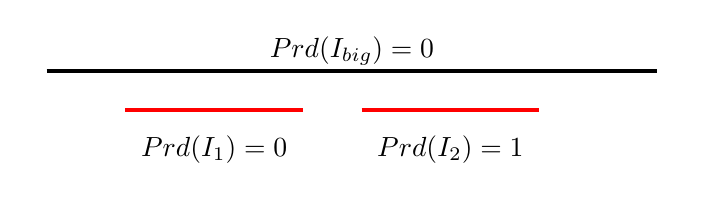
\begin{tikzpicture}[scale=0.5]
	
	\node at (0,0.5) {$Prd(I_{big}) = 0$};
	\node[draw=none] (I1a) at (-8,0) {$ $};
	\node[draw=none] (I1b) at (8,0) {$ $};
	\draw[line width=0.5mm] (I1a) -- (I1b);

	\node[draw=none] (I5a) at (-6,-1) {$ $};
	\node[draw=none] (I5b) at (-1,-1) {$ $};
	\node at (-3.5,-2) {$Prd(I_{1})=0$};
	\draw[color=red,line width=0.5mm] (I5a) -- (I5b);

 \node[draw=none] (I6a) at (0,-1) {$ $};
	\node[draw=none] (I6b) at (5,-1) {$ $};
	\node at (2.5,-2) {$Prd(I_{2})=1$};
	\draw[color=red,line width=0.5mm] (I6a) -- (I6b);

	\end{tikzpicture} 
        \caption{Instance of theorem \ref{theo:unw-naive-neg}.}
        \label{fig:neg-unit-irrev}
    \end{figure}
\end{proof}

\begin{corollary}
    Algorithm Naive is optimal for unit weights in the model of irrevocable acceptances.
\end{corollary}
Boyar et al. \cite{boyar2023online} were the first to consider the problem of interval selection with unit weights and irrevocable decisions, and they get the same (syntactically) performance, using a different algorithm, and a different set of predictions and error measure. In comparing our result to theirs, we note that our predictions are information theoretically strictly weaker than theirs\footnote{Their predictions consist of the entire input instance given in advance.}, and can in fact easily be extracted from theirs, allowing our algorithms to operate in their model. Furthermore, their predictions-following algorithm is enhanced with a \textit{greedy} aspect in order to achieve this optimal performance. As we will see in section \ref{section:exp}, experimental results on real-world data suggest that for some error ranges, pure \textit{greediness} is arguably a more important attribute than the use of predictions for getting a good solution, and the combination of both in the context of revocable acceptances works best.\\\\

We will now show that with \textbf{proportional weights}, algorithm \texttt{Naive} achieves the same performance bounds as in the case of unit weights.

\begin{theorem}
Algorithm Naive achieves $ALG \geq OPT - \eta$ for interval selection with proportional weights.
    \label{theo:prop-naive-pos}
\end{theorem}
\begin{proof}
        Without loss of generality, we assume integral lengths of intervals, and later explain how to generalize to real lengths. We discretize the weight of intervals into weight units, and define a weight element $w$ for each unit of weight. Let $W_{I} = \{w_{1},...,w_{w(I)}\}$ be the set of weight elements corresponding to the weight of interval $I$, with $W_{I} \cap W_{J} = \emptyset$ for any two distinct intervals $I,J$ . Let $W_{opt} = \bigcup_{I\in OPT}W_{I}$, and $W_{alg} = \bigcup_{I\in ALG}W_{I}$. The sets $H$ and $H_{I}$ are defined as for the unweighted algorithms. Lastly, let $C_{opt}(I)$ be the set of optimal intervals in $OPT$ that conflict with interval $I$.\\\\
    We argue for the existence of an injective mapping $F: W_{opt} \rightarrow W_{alg} \cup H$ as follows: Let $I_{opt}$ be an optimal interval. If $I_{opt}$ is taken by the algorithm, we map the elements of $W_{I_{opt}}$ to their corresponding elements in $W_{alg}$. If $I_{opt}$ is not taken by the algorithm, there are two cases. The first case is that $I_{opt}$ did not conflict with any interval in the solution, but $Prd(I_{opt}) = 0$. In this case, we know that $\eta(I_{opt}) = |H_{I_{opt}}| = w(I_{opt})$, and we can map the weight elements of $I_{opt}$ to error elements in $H_{I_{opt}}$.\\\\
    The other case is that $I_{opt}$ conflicted with at least one interval in the solution. Let that conflicting interval be $I_{c}$. It could also be that $Prd(I_{opt}) = 0$, and $H_{I_{opt}}$ would have error elements we can use, but we will assume the worst case of $Prd(I_{opt}) = 1$. In this case, it could be  $|W_{I_{opt}}| >  |H_{I_{c}}|$, and we cannot map the weight elements to error elements exclusively. We can, however, map the optimal weight elements, to elements in $H_{I_{c}} \cup W_{I_{c}}$. To see that there will always be sufficiently many unmapped elements, notice that $|H_{I_{c}} \cup W_{I_{c}}| \geq |\bigcup_{I \in C_{opt}(I_{c})}W_{I}|$. This is because $|H_{I_{c}}| = |\bigcup_{I \in C_{opt}(I_{c})}W_{I}| - |W_I|$, and $W_{I_c} \cap H_{I_c} = \emptyset$ always holds. We conclude that $|W_{alg}| + |H| \geq |W_{opt}|$, and we get the desired bound.\\\\
    To adapt the proof to real lengths, instead of considering sets of error and weight elements, we can define a transport plan using two transport matrices $H$ and $W$ of size $OPT\times ALG$. $H_{ij}$ (respectively $W_{ij}$) corresponds to the (real) amount of weight, or mass, mapped from $I_i \in OPT$ to the amount of error (resp. weight) introduced by $I_j \in ALG$. We can define these matrices such that for $1 \leq i \leq OPT$, $\sum_{1\leq j \leq ALG} H_{ij} + W_{ij} = w(I_i)$, for $1\leq j \leq ALG$, we have that $\sum_{1\leq i \leq OPT}H_{ij} \leq \eta(I_j)$ and $\sum_{1\leq i \leq OPT}W_{ij} \leq w(I_j)$.
\end{proof}
\begin{theorem}
For every deterministic algorithm, there exist a proportional weights instance and predictions, such that $ALG = OPT - \eta$.
    \label{theo:prop-naive-neg}
\end{theorem}
\begin{proof}
    Let $I_{1}$ arrive first with $Prd(I_{1}) = 0$. If the algorithm doesn't accept $I_{1}$, no more intervals arrive, and we have that $ALG = 0$, $OPT = w(I_{1})$, and $\eta = w(I_{1})$. If the algorithm accepts $I_{1}$, let two intervals $I_2$ and $I_3$ arrive next, with $w(I_2) = w(I_1)$, $Prd(I_2) = 1$, $w(I_3) = 2w(I_1)$ and $Prd(I_3) = 0$. In this case we have $ALG = w(I_1)$, $OPT = 3w(I_1)$, and $\eta = \eta(I_3) = 2w(I_1)$. In both cases the equality holds. One can repeat this construction for an asymptotic result.
\end{proof}

    \begin{figure}
	\centering
	
	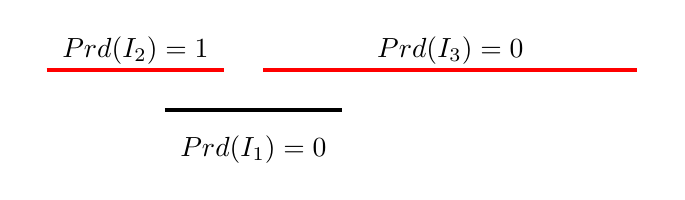
\begin{tikzpicture}[scale=0.5]

	\node at (-5,-2) {$Prd(I_{1}) = 0$};
	\node[draw=none] (I1a) at (-7.5,-1) {$ $};
	\node[draw=none] (I1b) at (-2.5,-1) {$ $};
	\draw[line width=0.5mm] (I1a) -- (I1b);
	
	
	%\node[draw=none] (d1) at (-3,-1) {$\rvdots$};

	
	\node[draw=none] (I3a) at (-10.5,0) {$ $};
	\node[draw=none] (I3b) at (-5.5,0) {$ $};
	\node at (-8,0.5) {$Prd(I_{2}) = 1$};
	\draw[color=red,line width=0.5mm] (I3a) -- (I3b);
	
	\node[draw=none] (I4a) at (-5,0) {$ $};
	\node[draw=none] (I4b) at (5,0) {$ $};
	\node at (0,0.5) {$Prd(I_{3}) = 0$};
	\draw[color=red,line width=0.5mm] (I4a) -- (I4b);

	\end{tikzpicture} 
	\caption{Instance of Theorem \ref{theo:prop-naive-neg}, with $w(I_2) = w(I_1), w(I_3) = 2w(I_1)$.}\label{fig:prop-neg-no-rev}
\end{figure}

\begin{corollary}
 Algorithm Naive is optimal for proportional weights in the model of irrevocable acceptances.
\end{corollary}